% LaTeX Article Template - customizing header and footer
\documentclass{article}

\newtheorem{thm}{Theorem}

% Set left margin - The default is 1 inch, so the following
% command sets a 1.25-inch left margin.
\setlength{\oddsidemargin}{0.25in}

% Set width of the text - What is left will be the right margin.
% In this case, right margin is 8.5in - 1.25in - 6in = 1.25in.
\setlength{\textwidth}{6in}

% Set top margin - The default is 1 inch, so the following
% command sets a 0.75-inch top margin.
\setlength{\topmargin}{-0.25in}

% Set height of the header
\setlength{\headheight}{0.1in}

% Set vertical distance between the header and the text
\setlength{\headsep}{0.2in}

% Set height of the text
\setlength{\textheight}{9in}

% Set vertical distance between the text and the
% bottom of footer
%\setlength{\footskip}{0.15in}

% Set the beginning of a LaTeX document
\usepackage{multirow}
\usepackage{xcolor,colortbl}
\usepackage{fullpage}
\usepackage{graphicx}
\usepackage{amsthm}
\usepackage{amssymb}
\usepackage{amssymb}
\usepackage{algpseudocode}
\usepackage{caption}
\usepackage{float}
\usepackage{subcaption}
\usepackage{fancyvrb}
\graphicspath{%
    {converted_graphics/}% inserted by PCTeX
    {/}% inserted by PCTeX
}

\definecolor{black}{rgb}{0,0,0}
%%%%%%%%%%%%%%%%%%%%%%%%%%%%%

\begin{document}\title{Graph Theory\\ Spring 2017\\ Math-M330}         % Enter your title between curly braces
\author{Steven Myers}        % Enter your name between curly braces
\date{\today}          % Enter your date or \today between curly braces
\maketitle


% Redefine "plain" pagestyle
\makeatother     % `@' is restored as a "non-letter" character

% Set to use the "plain" pagestyle
\pagestyle{plain}

\section*{Undirected and Directed Graphs}

\paragraph{}
Graphs are comprised of vertices and edges. An edge serves as a connection between two vertices. We can also say that if there is an edge between vertices, then there is a pathway to get from one vertex to the next. Some examples of where graphs are applicable are graphs forming relationships between locations. Some vertices under that example could be cities, and their edges would represent the roads or pathways that lead from one city to the next. There are two types of graphs: \textit{undirected} and \textit{directed}. A directed graph is one where edges have a direction. So, an edge from vertex $A$ to vertex $B$ means that there is a connection from $A$ to $B$, but not from $B$ to $A$. On the contrary, undirected graphs do not have direction, so an edge between two vertices is bidirectional. If we have an edge between two vertices $A$ and $B$, then there is a path from $A$ to $B$, and $B$ to $A$.\\

\begin{figure}[H]
    \centering
    \begin{minipage}{.45\textwidth}
        \centering
        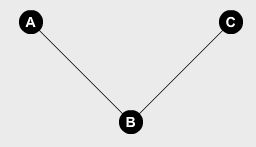
\includegraphics[width=.6\linewidth, height=.2\textheight]{undirected_graph}
        \caption{An undirected graph.}
    \end{minipage}
    \begin{minipage}{.45\textwidth}
        \centering
        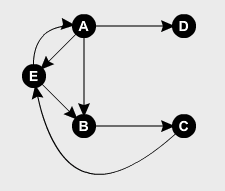
\includegraphics[width=.5\linewidth, height=.2\textheight]{directed_graph}
        \caption{A directed graph.}
    \end{minipage}
\end{figure}

\section*{Representing Graphs}
\paragraph{}
We can formally represent graphs as a collection of vertices and edges. A vertex is a singular point or constant, and an edge is tuple of two connected vertices. Two methods of concisely representing graphs in meaningful ways are \textit{adjacency matrices} and \textit{adjacency lists}. An adjacency matrix is a two dimensional array of boolean values. Its width and height are equal to the number of vertices in the graph, and every column and row represent a vertex. If the boolean value of some element at $(i,j)$ is true, then there is an edge from the vertex from row $i$ and a column $j$. This particular representation of a graph is useful only in undirected graphs, since there is no notion of direction. Adjacency matrices are symmetric, since the edges are undirected.\\\\

\begin{figure}[H]
\centering
\begin{subfigure}{.45\textwidth}
    \centering
    \begin{tabular}{|c|c|c|c|}
        \hline
         \cellcolor{black} & $A$ & $B$ & $C$\\
        \hline\hline
        $A$ & F & T & F\\
        \hline
        $B$ & T & F & T\\
        \hline
        $C$ & F & T & F\\
        \hline
    \end{tabular}
    \caption{An adjacency matrix for the graph in Figure 1.}
\end{subfigure}
\begin{subfigure}{.45\textwidth}
    \centering
    \begin{tabular}{|c||c|c|c|}
        \hline
        $A\rightarrow$ & $B$ & $D$ & $E$\\
        \hline
        $B\rightarrow$ & $C$ & & \\
        \hline
        $C\rightarrow$ & $E$ & &\\
        \hline
        $D\rightarrow$ & & &\\
        \hline
        $E\rightarrow$ & $A$ & $B$ &\\
        \hline
    \end{tabular}
    \caption{An adjacency list for the graph in Figure 2.}
\end{subfigure}
\end{figure}

\paragraph{}
Unlike adjacency matrices, an adjacency list is a convenient graphical representation for directed graphs in addition to undirected graphs. It consists of a unique set of all of the vertices of the graph, and for each vertex there is a list or vector of the vertices that particular vertex shares an edge with.

\section*{Euler Paths and Circuits}
\paragraph{}
We say that a graph is \textit{traversable} if every vertex is reachable from any other vertex. If a graph is traversable, then we know that every vertex in the graph can be visited. If a graph is traversable, and can be traversed by using every edge exactly once, then we say that the graph contains an Euler path. More precisely, an Euler path is a path in which every edge is traversed exactly once. A subset of Euler paths are Euler ciruits, which are Euler paths that begin and end on the same vertex.




\end{document}
